\section{Vulnerability scan}

\sectionframe

\frame{
	\frametitle{What we will do}

	\begin{columns}[T,onlytextwidth]
        \begin{column}{0.4\textwidth}
            We will:
            \begin{itemize}
                \item Explain VMs and vulnerable services
                \item Look at OpenVAS interface and tools
                \item Scan targets
				\item Look at a complete report
            \end{itemize}
        
		\end{column}
    \end{columns}
}


\frame{
	\frametitle{Debian VM}
	\begin{columns}[T,onlytextwidth]
        \begin{column}{0.4\textwidth}
            Vulnerable services
            \begin{itemize}
				\item Apache 
				\item CUPS
				\item FTP
				\item Samba
				\item SSH
				\item Syslog
            \end{itemize}
		\end{column}

		\begin{column}{0.5\textwidth}
            \centering
            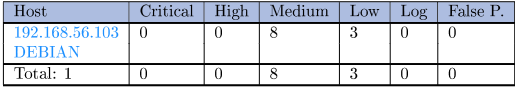
\includegraphics[width=\textwidth, height=0.4\textheight, keepaspectratio]{images/debian_vuln1.png}
            
            \vspace{0.5cm} % Adjust the gap between images here
            
            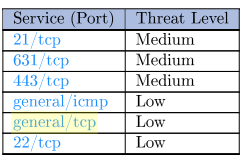
\includegraphics[width=\textwidth, height=0.3\textheight, keepaspectratio]{images/debian_vuln2.png}
        \end{column}

    \end{columns}
}

\frame{
	\frametitle{Windows XP}
	\begin{columns}[T,onlytextwidth]
        \begin{column}{0.4\textwidth}
            Vulnerable services
            \begin{itemize}
				\item FTP
				\item Firewall (inexsistent)
				\item General legacy things
            \end{itemize}
		\end{column}

		\begin{column}{0.5\textwidth}
            \centering
            \includegraphics[width=\textwidth, height=0.4\textheight, keepaspectratio]{images/Windows_vuln1.png}
            
            \vspace{0.5cm} % Adjust the gap between images here
            
            \includegraphics[width=\textwidth, height=0.3\textheight, keepaspectratio]{images/Windows_vuln2.png}
			\hfill
			\includegraphics[width=\textwidth, height=0.3\textheight, keepaspectratio]{images/Windows_vuln3.png}

        \end{column}
    \end{columns}
}

\frame{
	\frametitle{Excercise: Find out hosts IPs}
	Since we've configured a virtual network with DHCP IPs may vary, so you have to find them
	\begin{columns}[T,onlytextwidth]
        \begin{column}{0.4\textwidth}
            Vulnerable services
            \begin{itemize}
				\item On Windows: Open window from VirtualBox, open terminal and find IP via ipconfig /all
				\item On OpenVAS: Just see the IP on the top
            \end{itemize}
		\end{column}

		\begin{column}{0.5\textwidth}
            \centering
            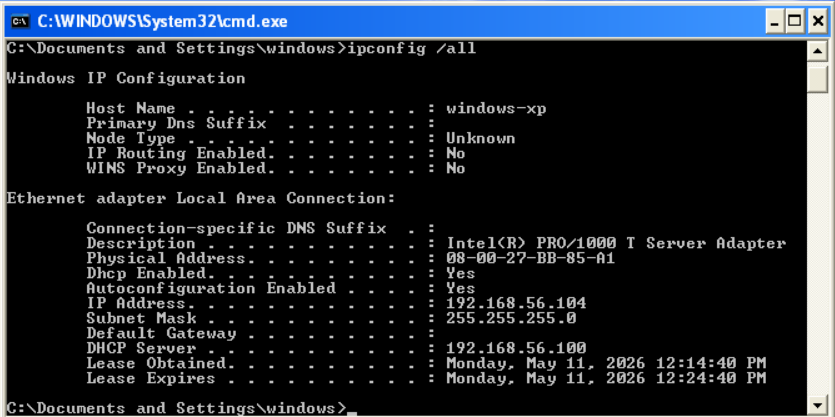
\includegraphics[width=\textwidth, height=0.4\textheight, keepaspectratio]{images/windowsxp_ipshow.png}

        \end{column}
    \end{columns}
}

